
\documentclass[aspectratio=169]{beamer}
\usepackage{tikz}
\usetikzlibrary{shadows,shapes.geometric,positioning,arrows,shapes.misc,shadings}

\tikzset{diagonal fill/.style 2 args={fill=#2, path picture={
			\fill[#1, sharp corners] (path picture bounding box.south west) -|
			(path picture bounding box.north east) -- cycle;}},
	Lemma/.style={rectangle, draw, rounded corners} , 
	Definition/.style={chamfered rectangle, draw} , 
	File/.style={rectangle,draw,text width=7.5em},
	FSM/.style={fill=blue!20},
	FSM_Product/.style={fill=yellow!20},
	ASC_LB/.style={fill=orange!20},
	ASC_Suite/.style={fill=lime!20},
	ASC_Sufficiency/.style={fill=lightgray!20},
	ASC_Hoare/.style={fill=magenta!20},
	line/.style = {draw, -latex'}
}


\begin{document}
\beamertemplatenavigationsymbolsempty

\begin{frame}{Overview of the correctness proof}


\begin{figure}
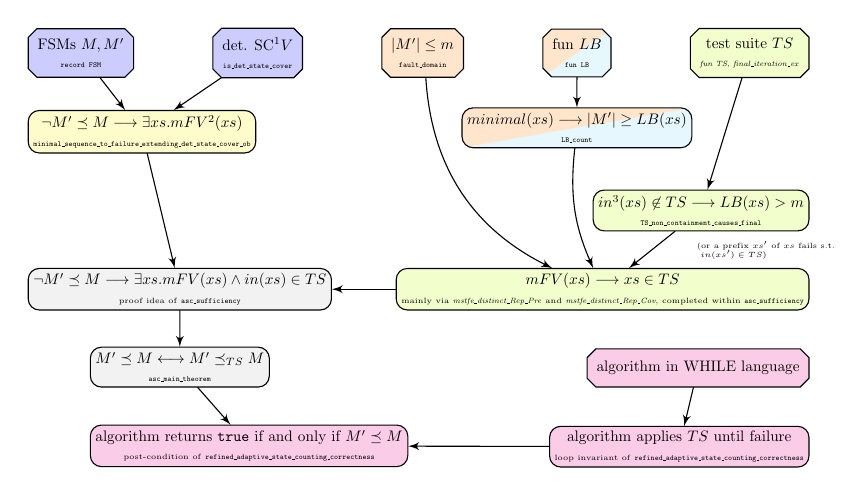
\begin{tikzpicture}[node distance = 1cm, auto, every node/.style={scale=0.55, text badly centered, minimum height=2.5em, align=center}]

\onslide<+-> {
        \node [Definition,FSM, anchor=north]                            (FSMs)          {FSMs $M,M'$  \\ {\tiny \texttt{record FSM}}};
        \node [Definition,FSM, right=1cm of FSMs]                            (V)          {det. SC\footnotemark $V$ \\ {\tiny \texttt{is\_det\_state\_cover}}};
}
 
\onslide<+->{
        \node [Lemma,FSM_Product, below=1 cm of FSMs.west, anchor=west]                        (mFV_ex)         {$\neg M' \preceq M \longrightarrow \exists xs . mFV\footnotemark(xs)$ \\ {\tiny \texttt{minimal\_sequence\_to\_failure\_extending\_det\_state\_cover\_ob}} };
        \path [line] (FSMs)         --                              (mFV_ex); 
        \path [line] (V)         --                              (mFV_ex);   
}
\onslide<+->{
        \node [Definition,ASC_LB, right=1cm of V]                            (SizeAssm)          {$|M'| \leq m$ \\ {\tiny \texttt{fault\_domain}}};
        \node [Definition,diagonal fill={cyan!10}{orange!20}, right=1cm of SizeAssm]                            (LB)          {fun $LB$ \\ {\tiny \texttt{fun LB}}};
}
\onslide<+->{
        \node [Lemma,diagonal fill={cyan!10}{orange!20}, below=1cm of LB.north]                            (minLB)          {$minimal(xs) \longrightarrow |M'| \geq LB (xs)$ \\ {\tiny \texttt{LB\_count}}};
        \path [line] (LB)         --                              (minLB);   
}
\onslide<+->{
        \node [Definition,ASC_Suite, right=1cm of LB.east, anchor=west]                            (TS)          {test suite $TS$ \\ {\tiny \textit{fun TS, final\_iteration\_ex}}};
}
\onslide<+->{
        \node [Lemma,ASC_Suite, below=2cm of TS.east, anchor=east,label={[align=left,shift={(1.5,-1.85)}]\tiny{(or a prefix $xs'$ of $xs$ fails s.t.} \\[-0.6em] \tiny{ $in(xs') \in TS$)}}]                            (elemTS)          {$in\footnotemark(xs) \not\in TS \longrightarrow LB(xs) > m$ \\ {\tiny \texttt{TS\_non\_containment\_causes\_final}}};
        \path [line] (TS)         --                              (elemTS);   
}
\onslide<+->{
        \node [Lemma,ASC_Suite, below=1cm of elemTS.east, anchor=east]                                                       (elemTSmin)          {$mFV(xs) \longrightarrow xs \in TS$ \\ {\tiny mainly via \textit{mstfe\_distinct\_Rep\_Pre} and \textit{mstfe\_distinct\_Rep\_Cov}, completed within \texttt{asc\_sufficiency} }};
        \path [line] (elemTS)         --                              (elemTSmin);   
        \path [line] (minLB)         edge[bend right=15]                              (elemTSmin);   
        \path [line] (SizeAssm)      edge[bend right]                                (elemTSmin);
}


\onslide<+->{
        \node [Lemma,ASC_Sufficiency, below=2cm of mFV_ex.west, anchor=west]                            (9)          {$\neg M' \preceq M \longrightarrow \exists xs . mFV(xs) \wedge in(xs) \in TS$ \\ {\tiny proof idea of \texttt{asc\_sufficiency}}};
        \path [line] (mFV_ex) -- (9);   
        \path [line] (elemTSmin) -- (9); 
}

\onslide<+->{
        \node [Lemma,ASC_Sufficiency, below=1cm of 9.north]                            (10)          {$M' \preceq M \longleftrightarrow M' \preceq_{TS} M$ \\ {\tiny \texttt{asc\_main\_theorem}}};
        \path [line] (9) -- (10);
}
\onslide<+->{
        \node [Definition,ASC_Hoare, below=2cm of elemTS.east, anchor=east]                            (11)          {algorithm in WHILE language};
}
\onslide<+->{
        \node [Lemma,ASC_Hoare, below=1cm of 11.east, anchor=east]                            (12)          {algorithm applies $TS$ until failure \\ {\tiny loop invariant of \texttt{refined\_adaptive\_state\_counting\_correctness}}};
        \path [line] (11) -- (12);
}
\onslide<+->{
        \node [Lemma,ASC_Hoare, below=1cm of 10.west, anchor = west]                            (13)          {algorithm returns \texttt{true} if and only if $M' \preceq M$ \\ {\tiny post-condition of  \texttt{refined\_adaptive\_state\_counting\_correctness}}};
        \path [line] (10) -- (13);
        \path [line] (12) -- (13);
}


\end{tikzpicture}
\hspace{0.2cm}
\vrule{}
\hspace{0.2cm}
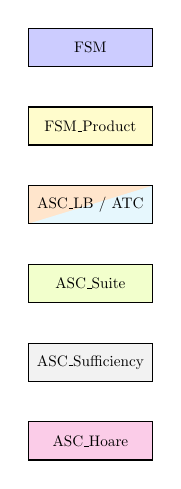
\begin{tikzpicture}[node distance = 1cm, auto, every node/.style={scale=0.55, text badly centered, minimum height=2.5em}]
        % Step 1
        \node [FSM,File]                            (FSM_File)          {FSM};
\onslide<2->{
        \node [FSM_Product,File, below=1cm of FSM_File.north]                        (FSM_Product_File)         {FSM\_Product};
}
\onslide<3->{
        \node [diagonal fill={cyan!10}{orange!20},File, below=1cm of FSM_Product_File.north]                        (ASC_LB_File)         {ASC\_LB / ATC};
}
\onslide<5->{
        \node [ASC_Suite,File, below=1cm of ASC_LB_File.north]                        (ASC_Suite_File)         {ASC\_Suite};
}
\onslide<8->{
        \node [ASC_Sufficiency,File, below=1cm of ASC_Suite_File.north]                        (ASC_Sufficiency_File)         {ASC\_Sufficiency};
}
\onslide<10->{
        \node [ASC_Hoare,File, below=1cm of ASC_Sufficiency_File.north]                        (ASC_Hoare_File)         {ASC\_Hoare};
}

\end{tikzpicture}
\end{figure}

\footnotetext[1]<1->{det. SC = deterministic state cover of $M$}
\footnotetext[2]<2->{mFV = minimal sequence to failure extending $V$}
\footnotetext[3]<6->{in = input portion}
\end{frame}


\end{document}